\documentclass{article}

\usepackage{graphicx}
\usepackage[utf8]{inputenc}
\usepackage[T1]{fontenc}
\usepackage[portuguese]{babel}

\newcommand{\tit}[1]{\textit{#1}}

\begin{document}

\title{Gerador de FFT (Fast Fourier Transform) em Tempo Real}
\author{Esdras R. Carmo, Gabriel R. Hioki}

\maketitle
\newpage
\tableofcontents
\newpage

\section{Introdução}


   A Transformada de Fourier Rápida (FFT) é um algoritmo que recebe um sinal
$x_n$ de amostras no domínio do tempo e retorna o vetor $X_m$ com os coeficientes
das funções senoidais em diferentes frequências. Em outras palavras, o FFT irá 
transformar um sinal no domínio do tempo para o domínio da frequência.

O FFT realiza otimizações no básico DFT (Discrete Fourier Transform) que consiste na seguinte
transformação linear:
$$
    X_m = \sum_{n=0}^{N-1}x_n w^{nm}
$$
onde $N$ é o tamanho dos vetores, $w = e^{2i\pi/N}$ são os fatores de rotação (\tit{twiddle}) e
$0 \leq m < N$. 

Uma FFT calcula rapidamente uma sequência dessas transformações fatorizando a matriz DFT em um produto de fatores esparsos. Como resultado, ele consegue reduzir a complexidade de calcular a DFT de  $N^2$ operações, para uma complexidade menor, de $N \log N$ operações \cite{fft-hardware}.

O FFT são de grande importância em uma vasta gama de aplicações, de Processamento digital de sinais para a resolução de equações diferenciais parciais a algoritmos para multiplicação de grandes inteiros.

\section{Descrição}
	O sistema irá calcular uma FFT através da utilização de uma \tit{Butterfly Unit} que realiza uma conta para cada par de palavras. Esse processo ocorrerá em 5 iterações e armazenará cada resultado em uma RAM diferente. Depois o resultado será ilustrado através de uma gráfico de barras em um monitor VGA.
\subsection{Monitor VGA}
    Hardware responsável por mostrar o resultado do FFT através de um gŕafico de barras.
\subsection{Central de Processamento (CP)}
    Hardware responsável por escrever, quando o enable (\tit{we}) for verdadeiro, o resultado da conta feita pelo \tit{Butterfly Unit} no respectivo endereço de memória na RAM correta, sendo dado de escrita (\tit{data\_re\_in/data\_im\_in}) e o dado de leitura(\tit{data\_re\_in/data\_im\_in}) com partes real e imaginária. manipular os índices e prover o fator \tit{twiddle} para o BFU;
\subsection{Butterfly Unit (BFU)}
    Hardware responsável por realizar as contas com as palavras fornecidas pelo CP (\tit{a\_re\_in, a\_im\_in, b\_re\_in, b\_im\_in}) e com o fator de rotação , \tit{twiddle} (\tit{tw\_re\_in, tw\_im\_in}) para gerar o resultado (\tit{a\_re\_out, a\_im\_out, b\_re\_out, b\_im\_out}) e enviar para o CP;
\subsection{RAM (0 to 5)}
    Unidades de memória com capacidade de leitura e escrita. Cada uma armazena os dados de uma iteração do cálculo e a RAM 0 é a entrada inicial e o resultado estará na RAM 5 depois que o cálculo for feito. Capacidade para 32 palavras de memória de 16 bits.

\newpage

\section{Diagrama de Blocos}

\begin{figure}[h!]
  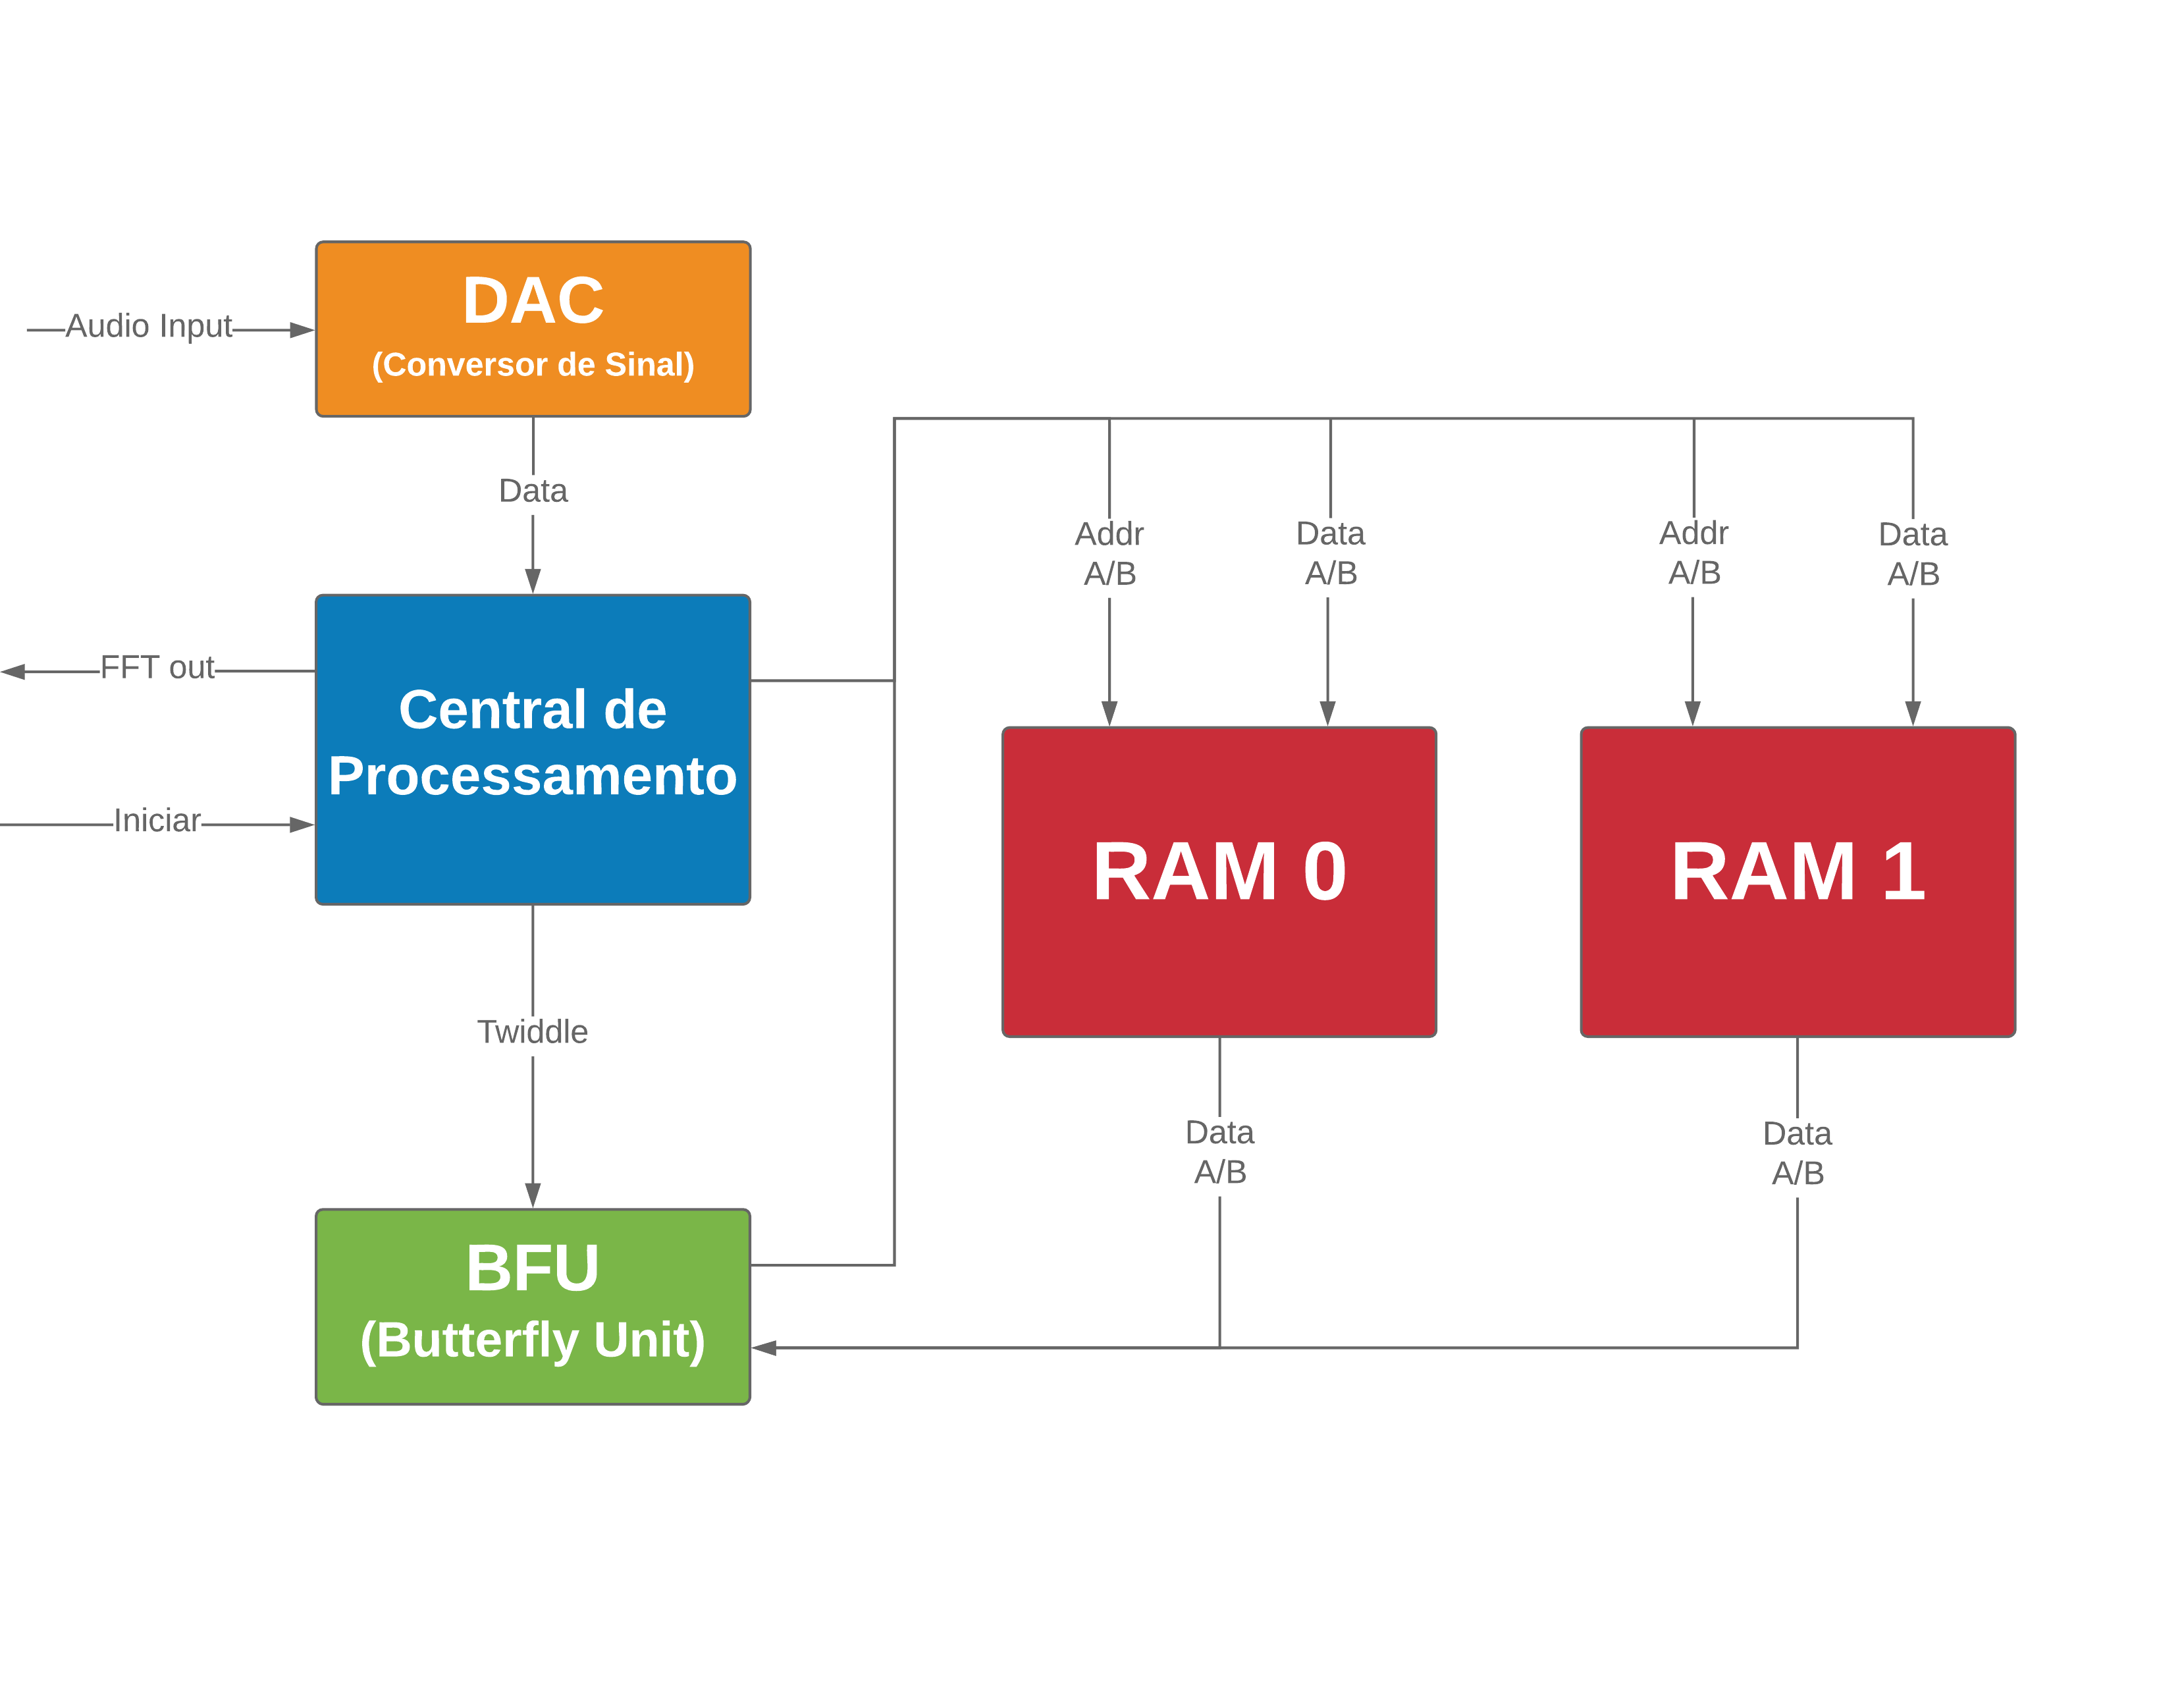
\includegraphics[width=\linewidth]{img/img.png}
  \caption{Diagrama de Blocos}
  \label{fig:diag}
\end{figure}

\newpage
\bibliography{doc}
\bibliographystyle{ieeetr}
\end{document}
